\documentclass[12pt]{beamer}
\usepackage{xeCJK}
\setCJKmainfont{蘋方-繁}
\renewcommand{\baselinestretch}{1.5}
\usepackage[T1]{fontenc}
\usetheme{CambridgeUS}
\usepackage[osf]{MinionPro}
\usepackage{MyriadPro}
\usecolortheme{beaver}

\newcommand*{\dif}{\,\mathrm{d}}
\newtheorem*{definition*}{Definition}
\newtheorem*{corollary*}{Corollary}
\def\tb#1#2{\mathop{#1\vphantom{\sum}}\limits_{\displaystyle #2}}
\usefonttheme{professionalfonts}

\usepackage{amsmath, amssymb, amsthm}
\newtheorem{prop}{\scshape Proposition}
\newenvironment{propc}[1]
{\begin{prop}}
        {\end{prop}}
\setbeamertemplate{theorems}[numbered]

\AtBeginSection[]{
  \begin{frame}
  \vfill
  \centering
  \begin{beamercolorbox}[sep=8pt,center,shadow=true,rounded=true]{title}
    \usebeamerfont{title}\insertsectionhead\par%
  \end{beamercolorbox}
  \vfill
  \end{frame}
}

\usepackage{tikz}
\usepackage{booktabs,tabulary}
\usepackage{threeparttable}

\title{R 語言教學}
\author{鍾旻錡, 陳柏瑜}
\institute[NTU Econ]{\scshape Statistics with Recitation  \\ NTU Econ}
\date{2020.12.23}

\begin{document}
\begin{frame}
\titlepage
\end{frame}

\begin{frame}
\frametitle{Outline}
\tableofcontents
\end{frame}


\section{Maximum Likelihood Estimation in R} 

%%%
\begin{frame}[fragile]{Concept of MLE}

Given random samples 
$$\{X_i\}_{i=1}^n \stackrel{i.i.d.}{\sim} f_X(x; \theta)$$

where $\theta$ is a unknown parameter

As long as $\theta$ is given, we can know the probability of seeing a certain outcome $x_i$


\end{frame}


%%%
\begin{frame}[fragile]{Concept of MLE}

To estimate $\theta$, we simply consider the converse relationship between random samples and their parameters.


$f_X(x_i; \theta)$ tells the probability of seeing a certain random outcome $x_i$ given $\theta$

$L(\theta ; x_i)$ tells the likelihood of a true parameter can be after we have seen a bunch of random samples $x_i$

\end{frame}


%%%
\begin{frame}[fragile]{D.G.P. and pseudo random numbers}

We can "make up" data in order to understand the Maximum Likelihood Estimation.

First, we pretend knowing the true parameters.

Second, generate a bunch of random numbers from the above process. (D.G.P.)

Third, we pretend not knowing the above information.

Fourth, write down the likelihood function according to the distribution function, and do the numerical maximization.

\end{frame}


%%%
\begin{frame}[fragile]{One Parameter}

D.G.P.

$$\{X_i\}_{i=1}^n \stackrel{i.i.d.}{\sim} Bernoulli(\mu)$$

where $n=100, \mu=0.87$


\end{frame}


%%%
\begin{frame}[fragile]{One Parameter}

The likelihood function is:

$$L(\mu) = \prod_{i=1}^n \mu^{x_i} (1-\mu)^{1-x_i}$$

$$\ell(\mu) = \sum_{i=1}^n x_i log(\mu) + \sum_{i=1}^n ({1-x_i}) log(1-\mu)$$

Note that "taking log" is essential for the computer to do the maximization problem.

\end{frame}


%%%
\begin{frame}[fragile]{One Parameter: Graph}

	\begin{figure}
		\begin{center}
			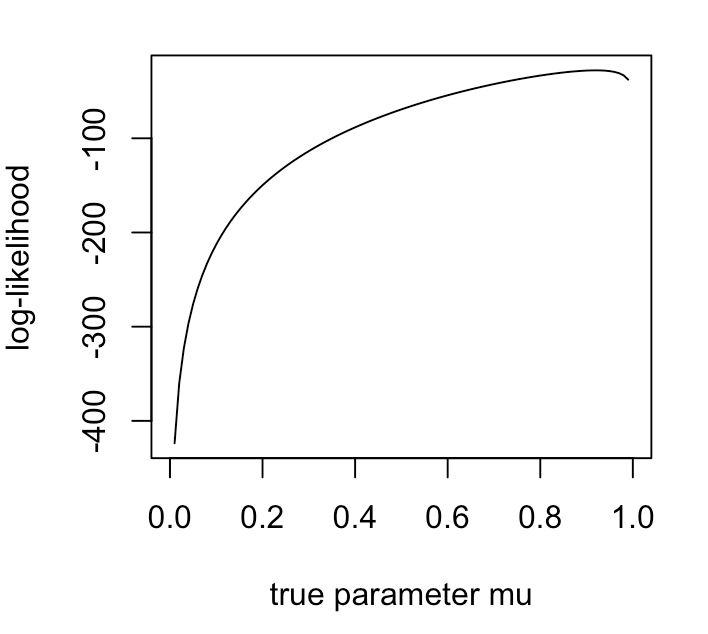
\includegraphics[width=0.6\textwidth]{figure/f01.png}
		\end{center}
	\end{figure}

\end{frame}


%%%
\begin{frame}[fragile]{One Parameter: Numerical Maximization}

In R, we can use $\texttt{`nlm()`}$ function to do the "non-linear minimization."

Alternatively, we can use $\texttt{`mle()`}$ in $\texttt{`stat4`}$ package.

The previous one provides one parameter estimation, while the latter one provides estimation for multiple parameters.

Other numerical maximization functions such as $\texttt{`optim()`}$ can also be used.

\end{frame}


%%%
\begin{frame}[fragile]{One Parameter: nlm() usage}

\texttt{nlm(objective function, staring points, print.level = 2, hessian = T)}

\begin{itemize}
	\item objective function: the function you want to minimize by deciding the variable $\theta$
	\item staring points: the initial value for $\theta$
	\item print.level: show all information for each iteration
	\item hessian: show the S.O.C.
\end{itemize}

\end{frame}


%%%
\begin{frame}[fragile]{One Parameter: Requirements to meet}

Remember that numerical maximization may highly depends on:

\begin{enumerate}
	\item starting points
	\item smoothness of the objective function
\end{enumerate}

And the iteration depends on:

\begin{enumerate}
	\item gradient (F.O.C.)
	\item Hessian (S.O.C.)
\end{enumerate}

\end{frame}

%%%
\begin{frame}[fragile]{One Parameter: Practice 1}

Given $$Pr(X=x) = f_X(x) = p(1-p)^x, x=0,1,2,3,\dots$$

Now, read the csv file $\texttt{practice1.csv}$ provided as the random samples.

Find the maximum likelihood estimate for $p$ with R

\end{frame}



%%%
\begin{frame}[fragile]{Two Parameters}

D.G.P.

$$\{Y_i\}_{i=1}^n \stackrel{i.i.d.}{\sim} N(\mu, \sigma^2)$$

where $n=100, \mu=0.9487, \sigma^2 = 9.487^2$

and $\texttt{`set.seed(1234)`}$


\end{frame}

%%%
\begin{frame}[fragile]{Two Parameters}

The likelihood function is:

\begin{verbatim}
mll = function(mu, sigma){
  logLikelihood <-0
  for(y in Y){
    logLikelihood <- logLikelihood + log(dnorm(y, mean = mu, sd = sigma))
  }
  return(-logLikelihood)
}
\end{verbatim}

\end{frame}


%%%
\begin{frame}[fragile]{Two Parameters: Graph}

	\begin{figure}
		\begin{center}
			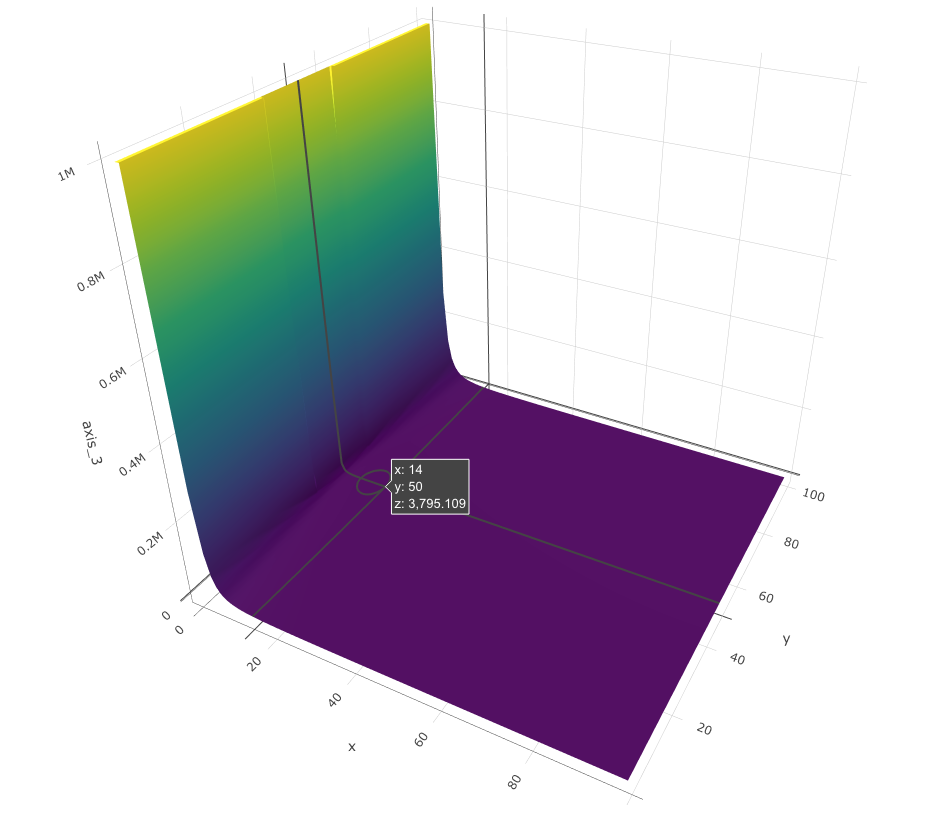
\includegraphics[width=0.6\textwidth]{figure/f02.png}
		\end{center}
	\end{figure}

\end{frame}

%%%
\begin{frame}[fragile]{Two Parameter: mle() usage}

$\texttt{mle(objective function, start)}$

\begin{itemize}
	\item objective function: the function you want to minimize by deciding the variable $\theta$
	\item start: a named list for $\theta$
\end{itemize}

\end{frame}


%%%
\begin{frame}[fragile]{Two Parameter: Practice 2}

Given $$\{X_i\}_{i=1}^n \stackrel{i.i.d.}{\sim} F(\nu_1, \nu_2)$$

Suppose the D.G.P. is:

$n = 10000$, $\nu_1 = 2020$, $\nu_2 = 1223$, and $\textt{set.seed(20201223)}$

Find the maximum likelihood estimate for $\nu_1, \nu_2$ with R

\end{frame}



\section{Interval Estimator and Interval Estimate}


%%%
\begin{frame}[fragile]{Interval Estimate}

Given
$$\{X_i\}_{i=1}^n \stackrel{i.i.d.}{\sim} Bernoulli(\mu)$$

the D.G.P. is:

$n=100, \mu = 0.87$

Construct the $(1-\alpha)100\%$ Interval Estimator / Estimate

\end{frame}


%%%
\begin{frame}[fragile]{Interval Estimate}

If $\alpha = 0.05$, then the interval estimate is:

$$ \bar{X}_n - z_{\frac{0.05}{2}} \frac{s_n}{\sqrt{n}}, \bar{X}_n + z_{\frac{0.05}{2}} \frac{s_n}{\sqrt{n}} $$

Write the above in R:

\begin{verbatim}
mean(X)-qnorm(0.975)*sd(X)/sqrt(n)
mean(X)+qnorm(0.975)*sd(X)/sqrt(n)
\end{verbatim}

\end{frame}


%%%
\begin{frame}[fragile]{Interval Estimator}

We may write a function that generates intervals by the same D.G.P., and then we can realize what "confidence" means.

\begin{verbatim}
confidence_interval = function(n=100, alpha=0.05){
  mu = 0.87
  X <- rbinom(n, size = 1, prob = mu)
  # qnorm(0.025); qnorm(0.975)
  l = mean(X)-qnorm(1-alpha/2)*sd(X)/sqrt(n)
  u = mean(X)+qnorm(1-alpha/2)*sd(X)/sqrt(n)
  return(c(l, u))
}\end{verbatim}

\end{frame}


%%%
\begin{frame}[fragile]{Interval Estimator}

	\begin{figure}
		\begin{center}
			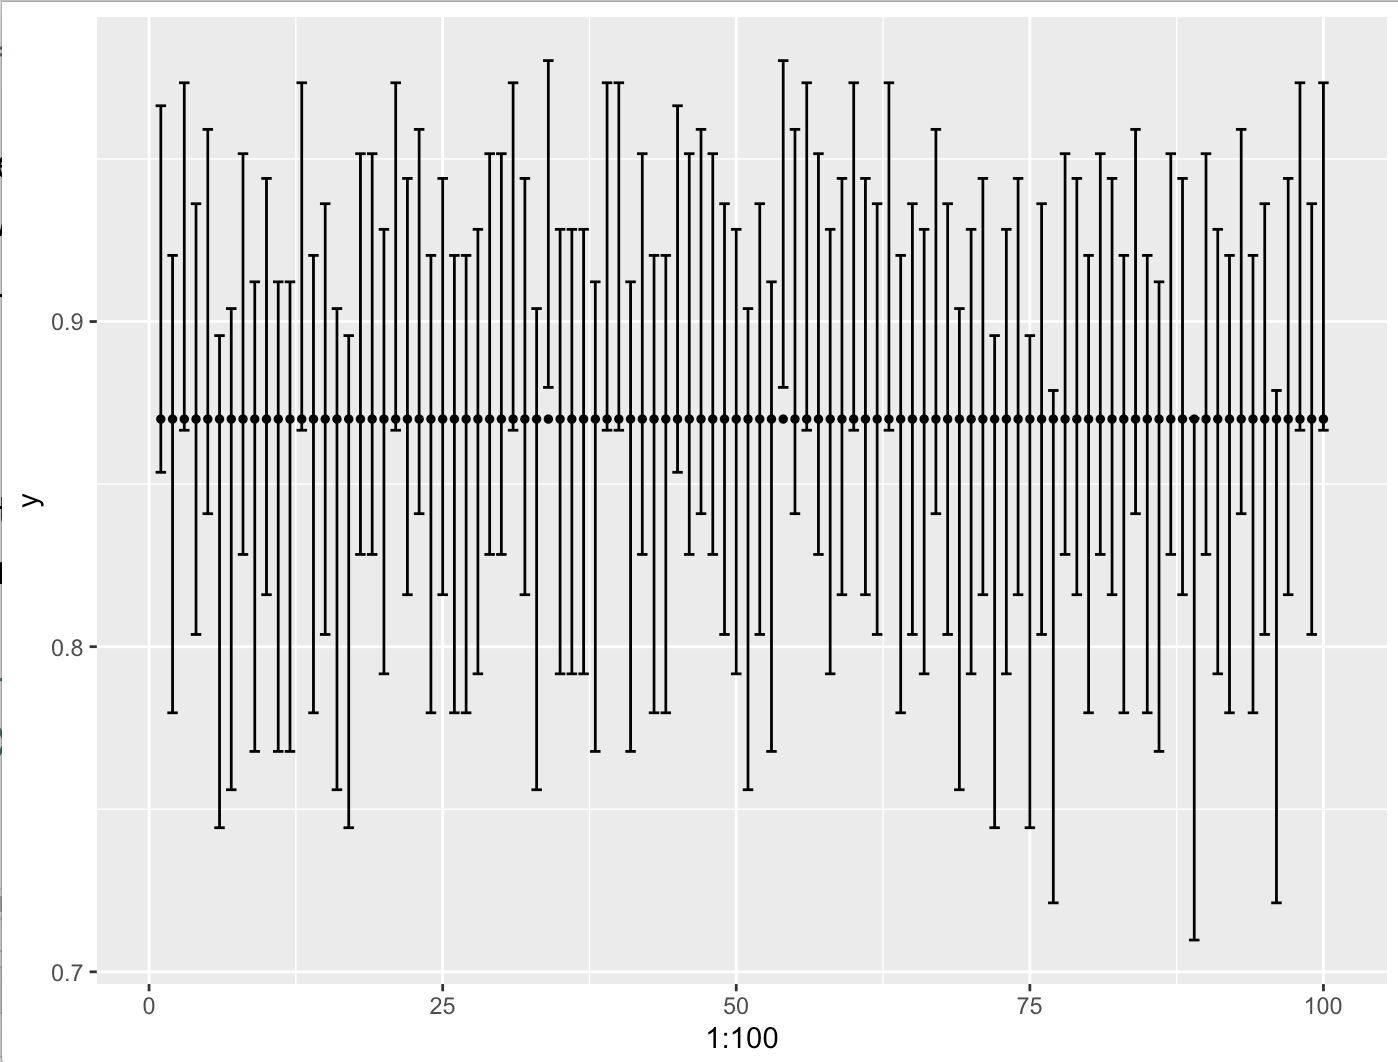
\includegraphics[width=0.6\textwidth]{figure/f03.png}
		\end{center}
	\end{figure}

\end{frame}



%%%
\begin{frame}[fragile]{Interval Estimate: Practice 3}

Consider
$$\{X_i\}_{i=1}^n \stackrel{i.i.d.}{\sim} N(\mu, \sigma^2)$$ where both $\mu, \sigma^2$ are unknown

Construct the 95\% Interval Estimate for $\sigma^2$

\end{frame}



\section{Hypothesis Test}


%%%
\begin{frame}[fragile]{Hypothesis Test: Two Aspects}

Given $\alpha$,

\begin{enumerate}
	\item Consider whether the parameter of interest is in the interval estimate I constructed
	\item Suppose null hypothesis is true, then how unlikely it is that I can see the realized random samples?
\end{enumerate}}

\end{frame}



%%%
\begin{frame}[fragile]{Hypothesis Test: Aspect 1}

Given
$$\{X_i\}_{i=1}^n \stackrel{i.i.d.}{\sim} Bernoulli(\mu)$$

the D.G.P. is:

$n=100, \mu = 0.87$

Construct the $(1-\alpha)100\%$ Interval Estimator / Estimate

\end{frame}


%%%
\begin{frame}[fragile]{Hypothesis Test: Aspect 1}

If someone claims: the true parameter $\mu$ is exactly $0.87$

What can we say depends on the realized random samples?

\end{frame}

%%%
\begin{frame}[fragile]{Hypothesis Test: Aspect 1}

	\begin{figure}
		\begin{center}
			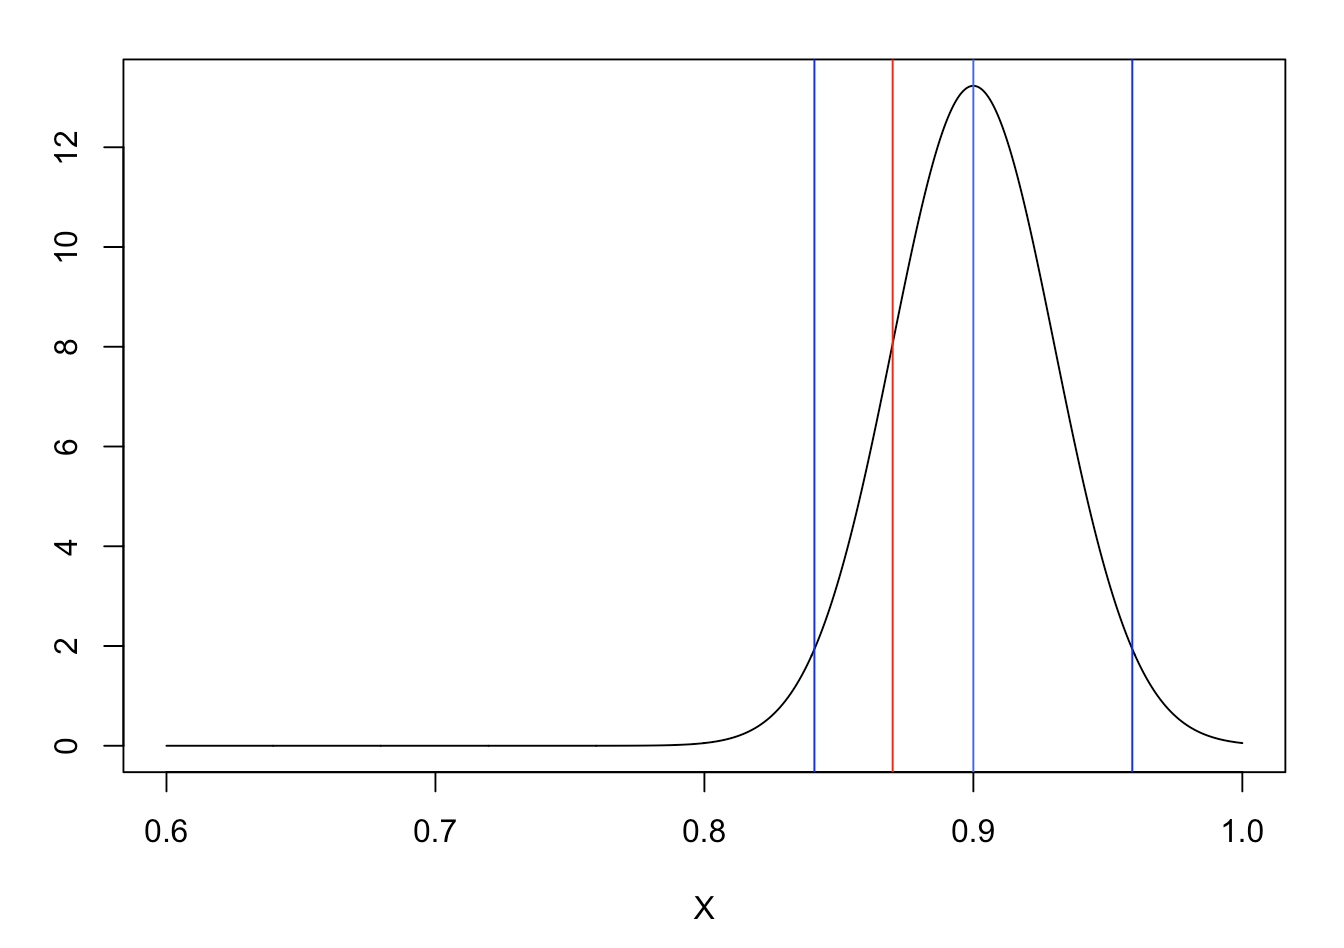
\includegraphics[width=0.6\textwidth]{figure/f04.png}
		\end{center}
	\end{figure}

Red: null hypothesis; Blue: random sample we saw
\end{frame}

%%%
\begin{frame}[fragile]{Hypothesis Test: Aspect 1}

	\begin{figure}
		\begin{center}
			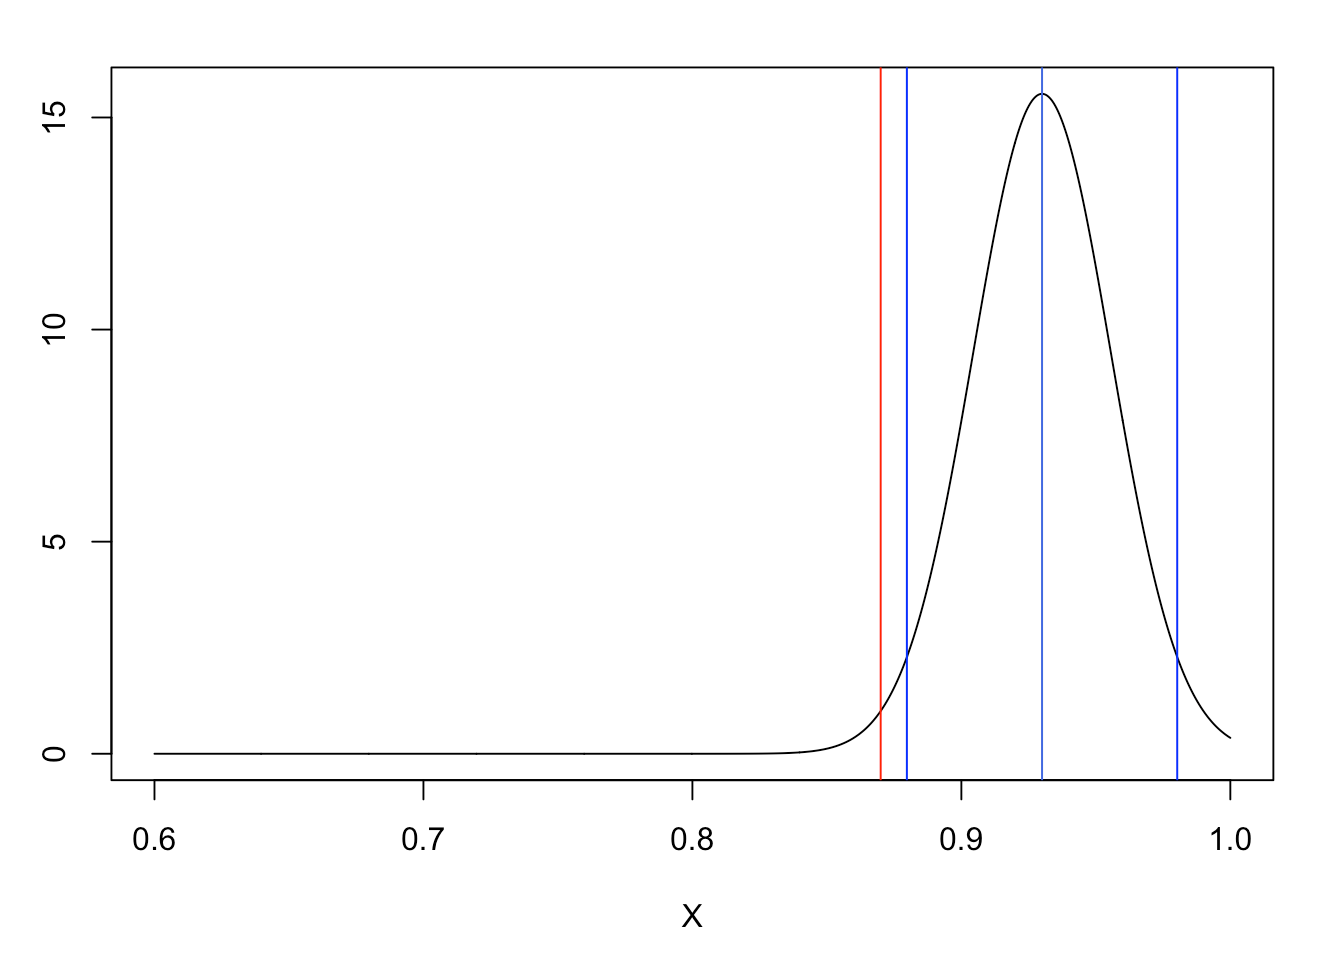
\includegraphics[width=0.6\textwidth]{figure/f05.png}
		\end{center}
	\end{figure}
Red: null hypothesis; Blue: random sample we saw
\end{frame}


%%%
\begin{frame}[fragile]{Hypothesis Test: Aspect 2}

If someone claims: the true parameter $\mu$ is exactly $0.87$

Now suppose what he said is true, then how could we verify his claim?

\end{frame}


%%%
\begin{frame}[fragile]{Hypothesis Test: Aspect 2}

	\begin{figure}
		\begin{center}
			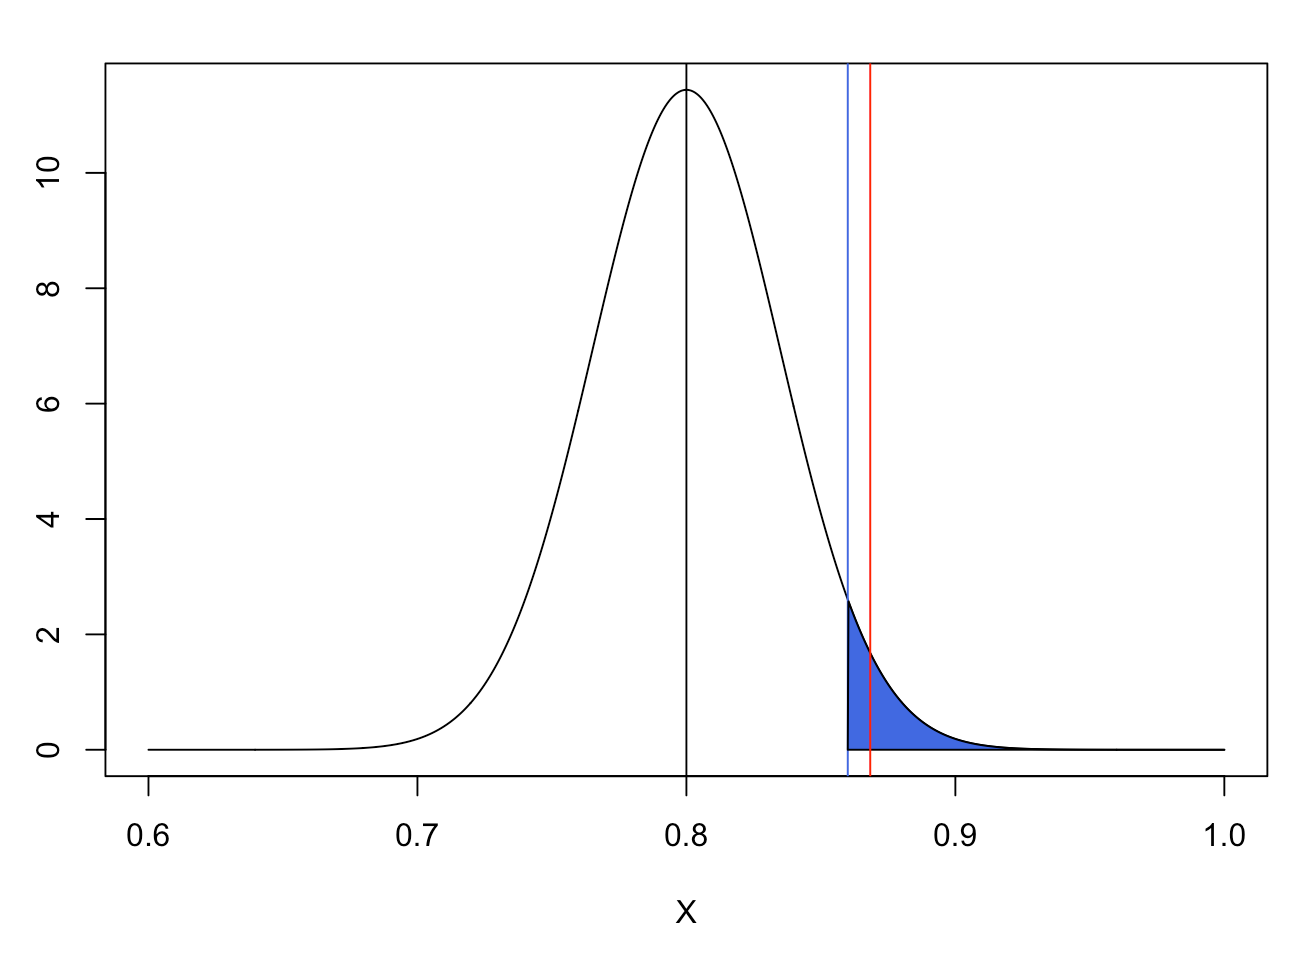
\includegraphics[width=0.6\textwidth]{figure/f06.png}
		\end{center}
	\end{figure}

Red: significance level 0.05; Blue: random sample we saw; Black: null hypothesis

\end{frame}


%%%
\begin{frame}[fragile]{Hypothesis Test: Aspect 2}

	\begin{figure}
		\begin{center}
			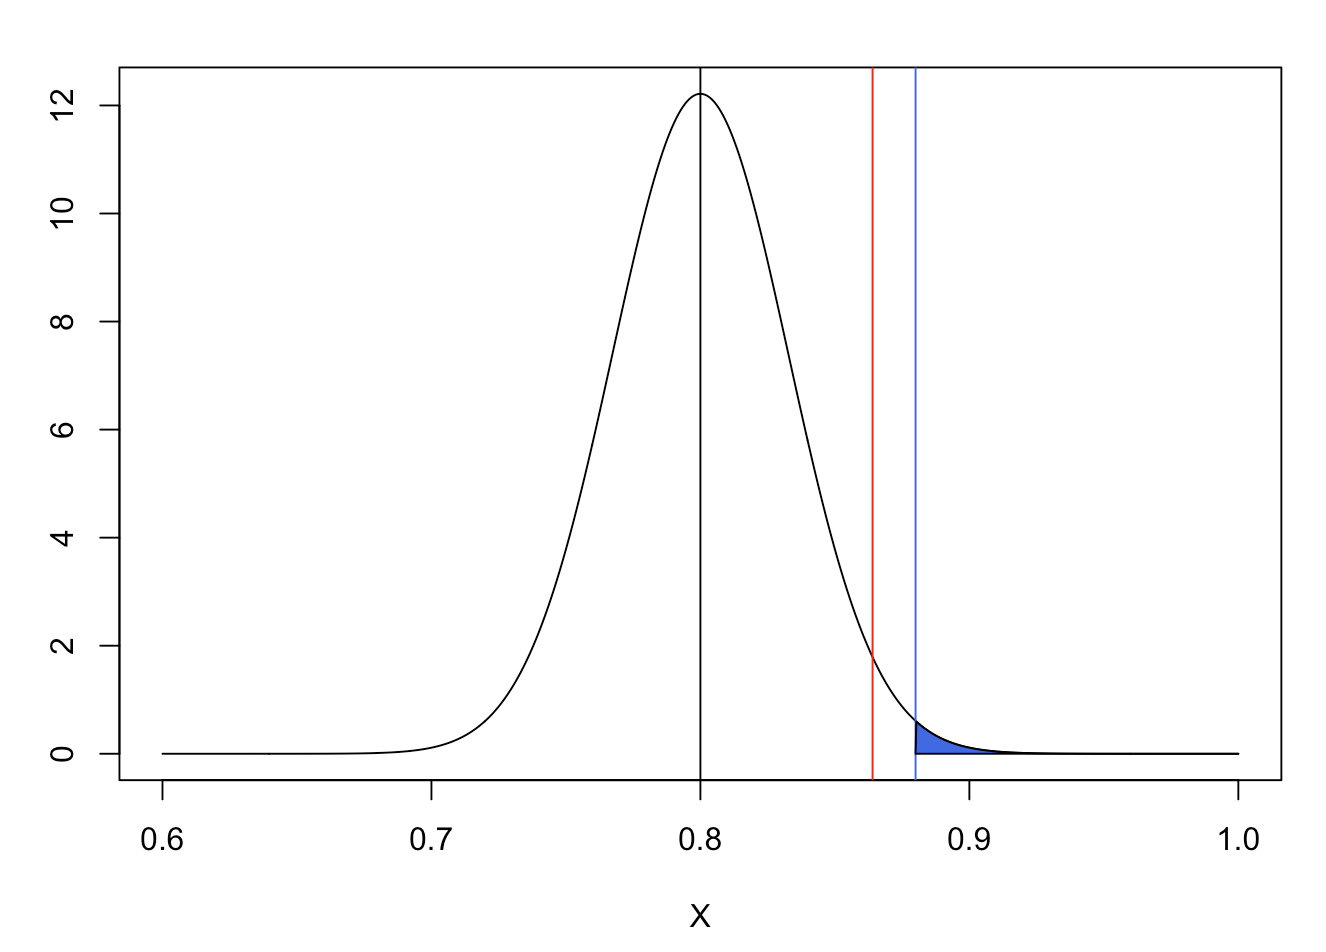
\includegraphics[width=0.6\textwidth]{figure/f07.png}
		\end{center}
	\end{figure}

Red: significance level 0.05; Blue: random sample we saw; Black: null hypothesis

\end{frame}


%%%
\begin{frame}[fragile]{Hypothesis Test: Practice 4}

Given $$\{X_i\}_{i=1}^n \stackrel{i.i.d.}{\sim} N(\mu, \sigma^2)$$

the D.G.P. is:

$n=10000, \mu = \pi, \sigma^2 = \pi$

$$H_0: \sigma^2 = 3$$
$$H_A: \sigma^2 \neq 3$$ 

Find the test statistics if $\alpha=0.05$

\end{frame}



\section{Permutation Test}

%%%
\begin{frame}[fragile]{An Alternative Approach of Hypothesis Test}

	\begin{itemize}
		\item Example in $\textbf{Mathematical Statistics with Re-sampling and R}$ Ch3.1 (Chihara)
		\item Scientists invent a new drug that supposedly will inhibit a mouse’s ability to run through a maze.
		\item The average time for the drug group is 25 s, and the average time for the control group is 20.33 s.
		\item The mean difference in times is 25 − 20.33 = 4.67 s.
	\end{itemize}}

	\begin{figure}
		\begin{center}
			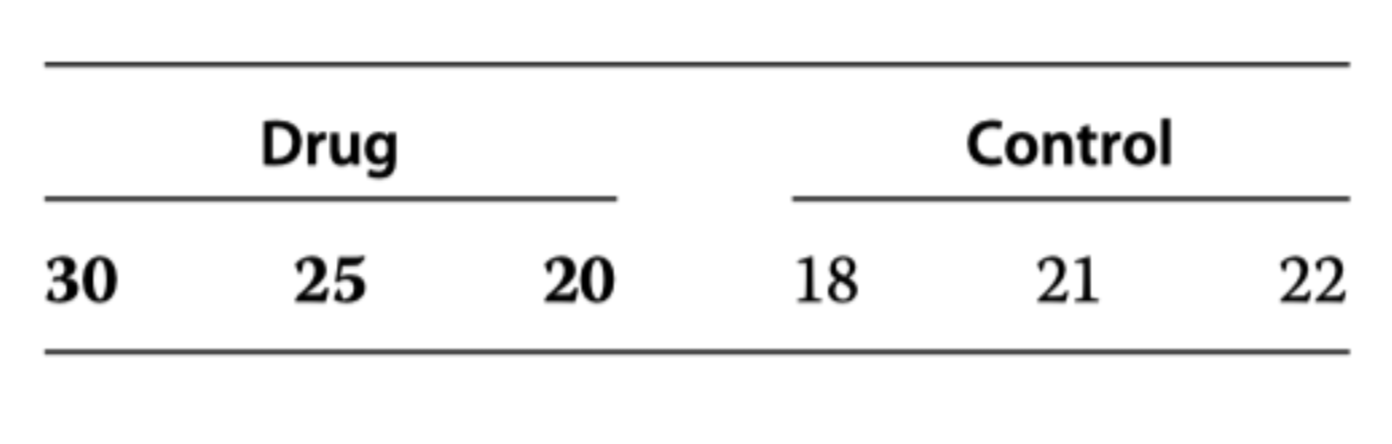
\includegraphics[width=0.5\textwidth]{figure/f08.png}
		\end{center}
	\end{figure}

\end{frame}


%%%
\begin{frame}[fragile]{An Alternative Approach of Hypothesis Test}

We cannot tell for sure whether there is a real effect. What we do instead is to estimate how easily pure random chance would produce a difference this large. If that probability is small, then we conclude there is something other than pure random chance at work, and conclude that there is a real effect.

If what we saw is:

	\begin{figure}
		\begin{center}
			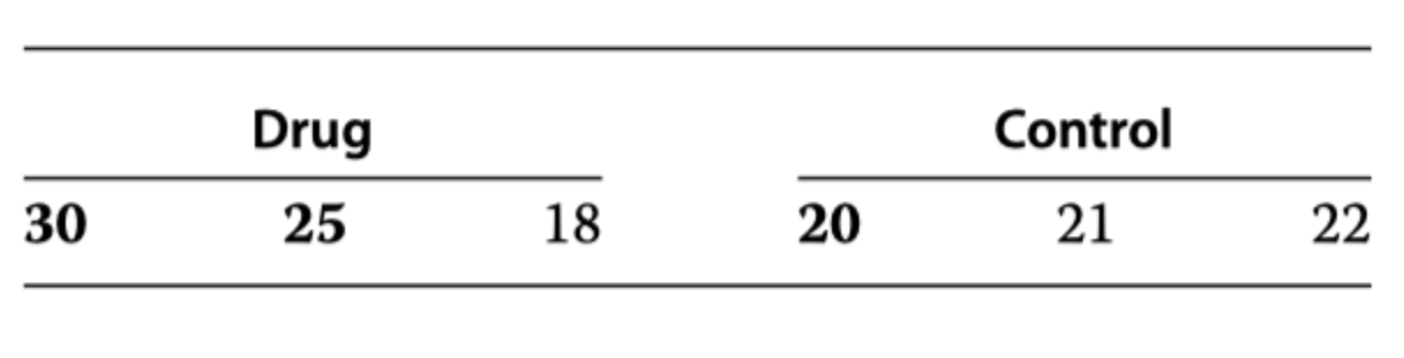
\includegraphics[width=0.6\textwidth]{figure/f09.png}
		\end{center}
	\end{figure}

\end{frame}


%%%
\begin{frame}[fragile]{An Alternative Approach of Hypothesis Test}

Original:
	\begin{figure}
		\begin{center}
			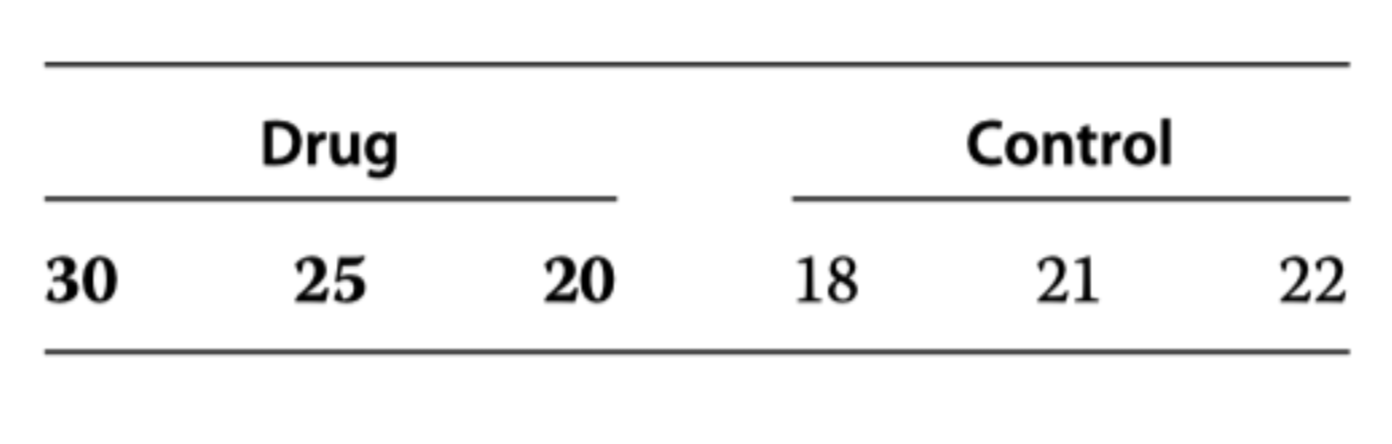
\includegraphics[width=0.6\textwidth]{figure/f08.png}
		\end{center}
	\end{figure}

After permutating:
	\begin{figure}
		\begin{center}
			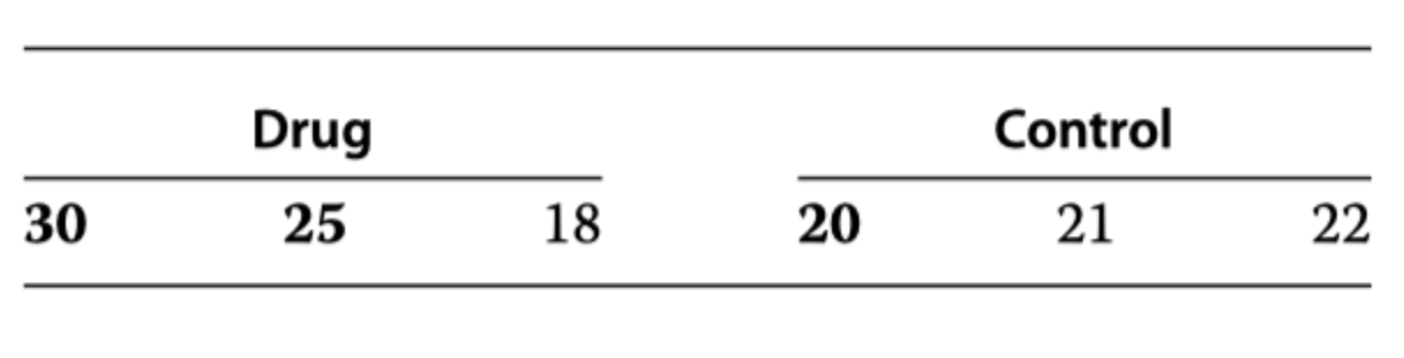
\includegraphics[width=0.6\textwidth]{figure/f09.png}
		\end{center}
	\end{figure}

There are ${6 \choose 3}$ combinations for these samples.

\end{frame}


%%%
\begin{frame}[fragile]{An Alternative Approach of Hypothesis Test}

	\begin{figure}
		\begin{center}
			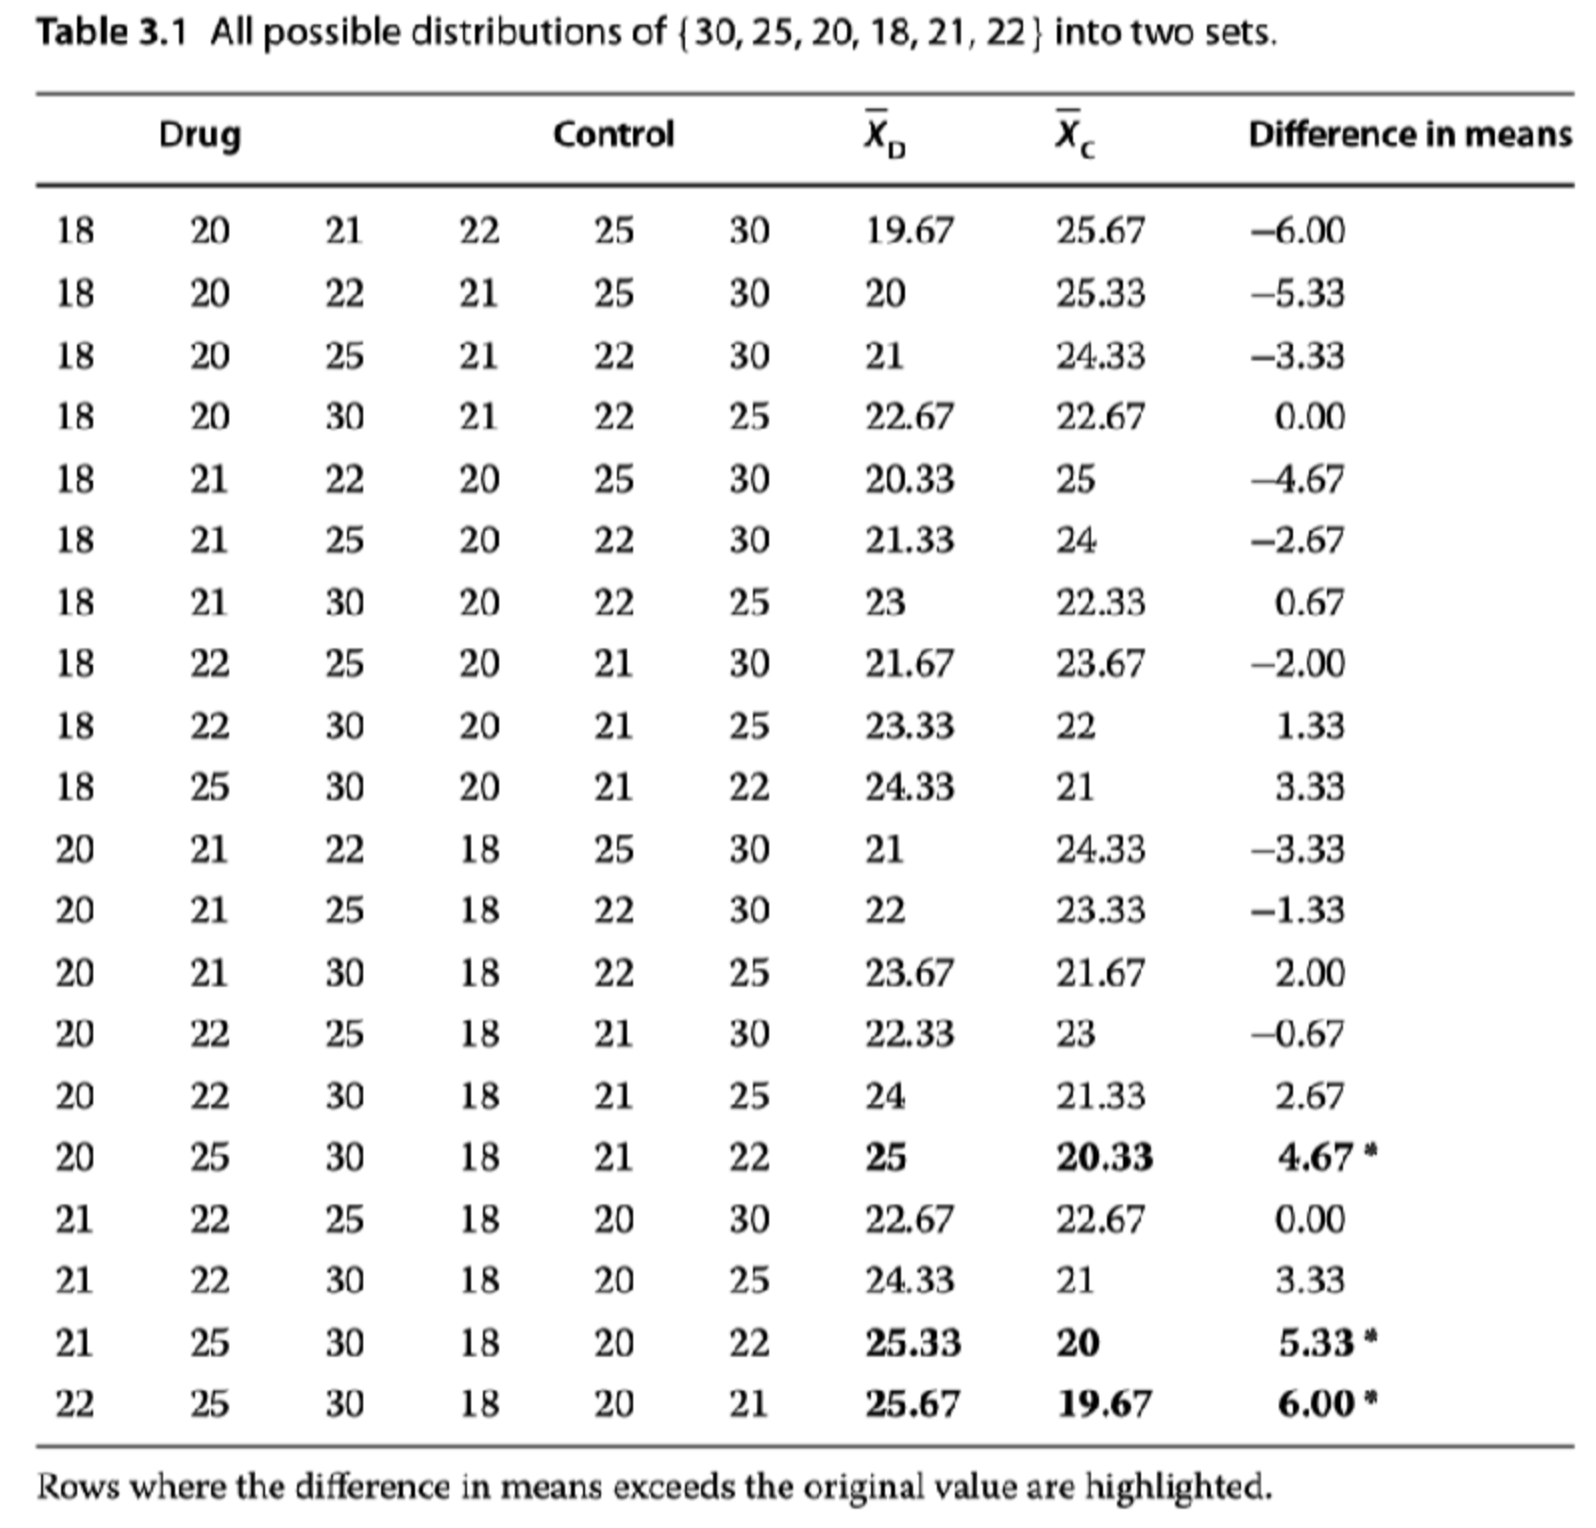
\includegraphics[width=0.6\textwidth]{figure/f10.png}
		\end{center}
	\end{figure}

\end{frame}


%%%
\begin{frame}[fragile]{An Alternative Approach of Hypothesis Test}

	\begin{itemize}
		\item Among 20 possible combinations, there are only 3 of them has a more extreme difference in sample mean. (compared to 4.67)
		\item $H_0:$ There is no difference between “Drug” group and “Control” group.(i.e. There is no effect on drug.)

		\item $H_A:$ There is a negative difference between “Drug” group and “Control” group.(i.e. There is an effect on drug that makes mice run through the maze faster.)
		\item The relative frequency of seeing a more extreme "difference in sample means" is the "p-value" under $H_0$
	\end{itemize}}

\end{frame}


%%%
\begin{frame}[fragile]{Is Permutation Feasible? Re-sampling!}

	\begin{itemize}
		\item Extend to $n$ mice, then there are ${n \choose \frac{n}{2}}$ combinations
		\item To calculate p-value, We need re-sampling
	\end{itemize}}

\end{frame}


%%%
\begin{frame}[fragile]{Permutation Test Example}

	\begin{itemize}
		\item Chihara Ch3.3
		\item Investigating the consumption of hotwings and beer in a bar, while recording the gender.
		\item Goal: Do men consume more hot wings than women?
	\end{itemize}}

	\begin{figure}
		\begin{center}
			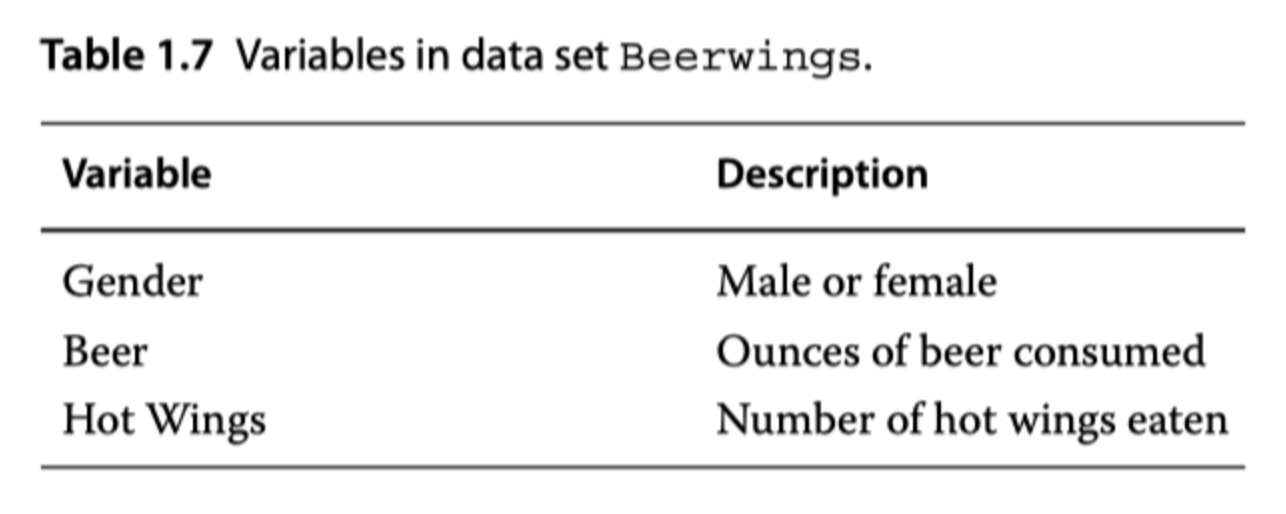
\includegraphics[width=0.6\textwidth]{figure/f11.png}
		\end{center}
	\end{figure}

\end{frame}


%%%
\begin{frame}[fragile]{Permutation Test Example}

	\begin{itemize}
		\item 30 observations
		\item $H_0:$ Gender does not affect the consumption of hot wings

		\item $H_A:$ Men do consume more hot wings.
		\item Under $H_0$, the following is one of the possible outcomes
	\end{itemize}}

	\begin{figure}
		\begin{center}
			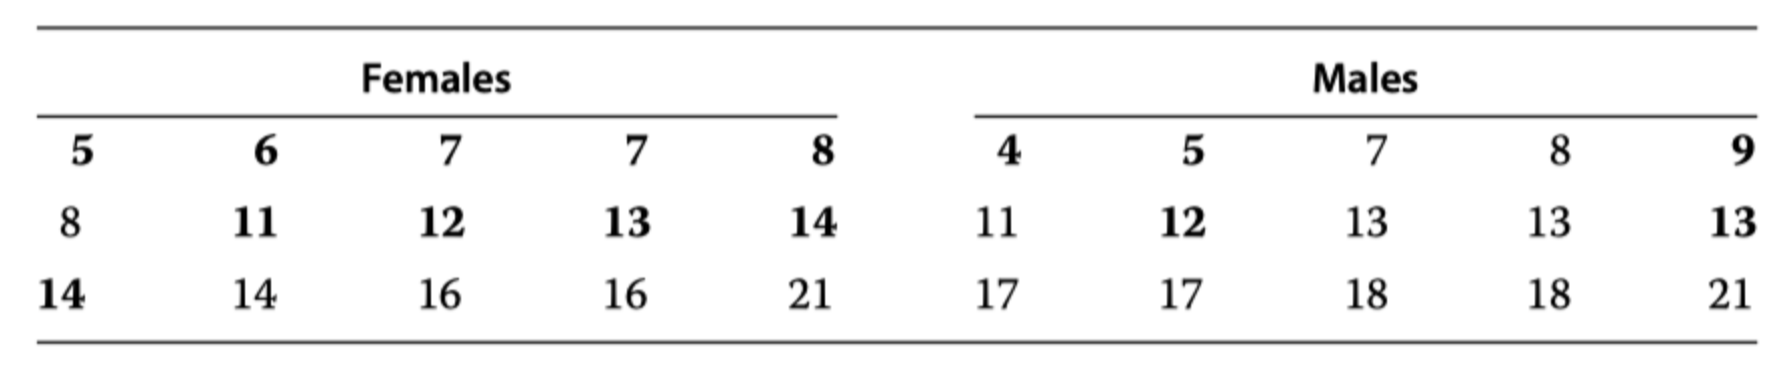
\includegraphics[width=0.6\textwidth]{figure/f12.png}
		\end{center}
	\end{figure}

	\begin{itemize}
		\item Note that there are ${30 \choose 15} = 155,117,520$ combinations under $H_0$
	\end{itemize}}

\end{frame}


%%%
\begin{frame}[fragile]{Permutation Test Example}

	\begin{itemize}
		\item We can create permutation resample since all possible outcomes are weighted with same probability.
		\item What we want is calculating p-value. We can draw some outcomes from the permutations and see whether they are extreme events or not.
		\item The number of extreme events over the number we draw
(which is the relative frequency) is the approximation of p- value.
	\end{itemize}}

\end{frame}


\section{}
\begin{frame}
\begin{center}
{\huge 感謝大家聆聽}
\end{center}
\end{frame}
\end{document}